
\documentclass[12pt,onecolumn]{IEEEtran}
%packages
\usepackage{cite}
\usepackage{gensymb}
\usepackage{amssymb,amsmath}
\usepackage{textcomp}
\usepackage{csquotes}
\usepackage{graphicx}
\usepackage{blindtext, graphicx}
\graphicspath{ {imgs/} }

\usepackage{dblfloatfix} 
% *** GRAPHICS RELATED PACKAGES ***
%
\ifCLASSINFOpdf
  % \usepackage[pdftex]{graphicx}
  % declare the path(s) where your graphic files are
  % \graphicspath{{../pdf/}{../jpeg/}}
  % and their extensions so you won't have to specify these with
  % every instance of \includegraphics
  % \DeclareGraphicsExtensions{.pdf,.jpeg,.png}
\else
  % or other class option (dvipsone, dvipdf, if not using dvips). graphicx
  % will default to the driver specified in the system graphics.cfg if no
  % driver is specified.
  % \usepackage[dvips]{graphicx}
  % declare the path(s) where your graphic files are
  % \graphicspath{{../eps/}}
  % and their extensions so you won't have to specify these with
  % every instance of \includegraphics
  % \DeclareGraphicsExtensions{.eps}
\fi

\hyphenation{op-tical net-works semi-conduc-tor}


\begin{document}
\title{Review on \\ Towards 1 Gbps/UE in Cellular Systems: Understanding Ultra-Dense Small Cell Deployments}
\author{\IEEEauthorblockN{Sai Narsi Reddy Donthi Reddy}\\
\IEEEauthorblockA{School of Computing and Engineering\\
University of Missouri -  Kansas City\\
Email: sdhy7@mail.umkc.edu\\
UMKC ID: 16186610}}
\maketitle



\section{Introduction}
\label{sec:intro}

With the on going advancements in smart devices, the number internet of things (IOT) had increased drastically in recent years. It is estimated that by 2020, the number of wireless smart devices connected to internet increase to $25$ Billion ~\cite{Gartner}. To meet this demands in ~\cite{main_paper} authors forecast that it requires at least $100$ folds increase in the network capacity. It is shown that this kind of increments can be achieved by using tool from three paradigms. Firstly, network densification. Secondly, higher frequency bands and Lastly, spectral efficiency enhancements using multi-antenna systems and scheduling techniques. 

Out of these three network densification plays the important role in improving the network capacity by increasing the number of cells in the network and reducing the size of the cell. From their simulation results it is shown that by considering $200m$ as the cell size and $100MHz$ as the bandwidth as the base line. These is a $7.56$ folds increment in network capacity by going down to $35m$ cell size and another $5$ folds increment using $10GHz$ carrier frequency with $500MHz$ as bandwidth. An another $2$ folds increment is possible by using beam-forming multi-antenna technology and achieving $1.27Gbps$ per User Equipment (UE). With small cell sizes scheduling techniques like proportional fair perform close to simple round robin technique due to increase in the multi-user diversity.

\section{Paper Outline}
\label{sec:PO}

 \renewcommand{\theenumi}{\Roman{enumi}}
 \begin{enumerate}
   \item Abstract
   \item Index Terms
   \item Introduction
   \item Small Cells in HetNets
   \item Why Are Today's Small Cells Not Practical to Meet Future Capacity Demands?
   \item System Model
   \item Network Densification
   \begin{enumerate}
     \item Idle Mode Capability and the 1 UE per cell concept
     \item Transmit Power and UE SINR Distribution
     \begin{enumerate}
     \item Transmit Power
     \item UE SINR Distribution
     \end{enumerate}
     \item Transition From the Interference-Limited Regime to the Noise-limited Regime
     \end{enumerate}
   \item Higher Frequency Bands
   \item Multi-antenna Techniques and Beamforming
   \item Scheduling
   \item Energy-Efficiency
   \item What is Different in Ultra-Dense Small Cell Deployments
   \item Challenges in Ultra-Dense Small Cell Deployments
   \item Conclusion
   \item Appendix
   \item References
 \end{enumerate}

\section{The Problem}
\label{sec:TP}
It is estimated that by 2020 at least 100 folds network capacity should be increase to meet the oncoming demand. Currently, vendors and operators are implementing different technologies to improve the network capacity. All the existing tools can be classified into three categories as show in figure - \ref{fig:NWCP}. First, increasing spatial reuse by network densification  which is been done by increasing type-3 small cells in a type-1 macro cells (HetNet architecture). Second, By exploring higher spectrum frequencies which gives higher bandwidth per cell. And lastly, more spectral efficiency by using multi-antenna system, dynamic TDD etc,. 

\begin{figure}[ht]
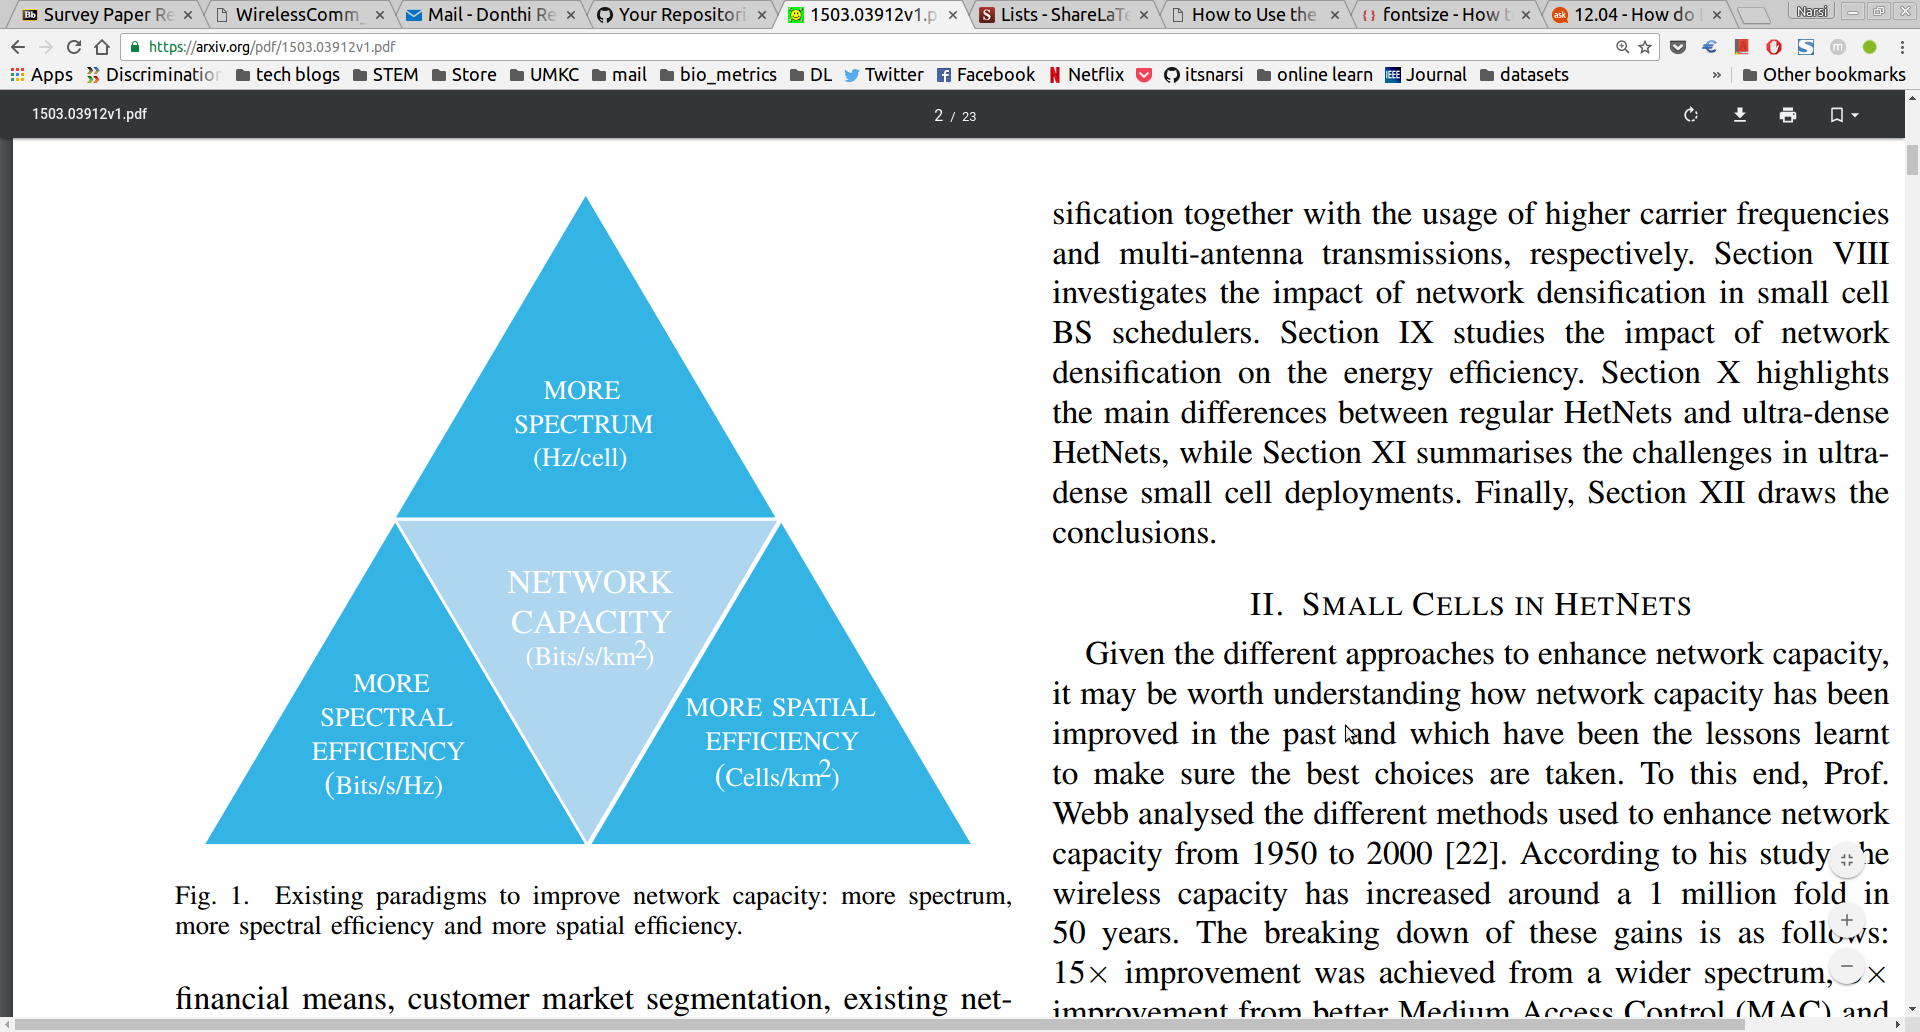
\includegraphics[scale=0.3]{nwcp_class}
\centering
\caption{Three categories of existing tools to improve Network capacity.~\cite{main_paper}}
\label{fig:NWCP}
\end{figure}
However, these improvements are not enough to meet the future demand. If small cell base station (BS) is close to macro cell tower as shown in figure - ~\ref{fig:SMI}, due to large difference in transmission power between macro cell and co-channel small cell (Type-2 cells), UE's tend to connect to macro cell base station (BS) rather than high speed small cell which in turn reduces the coverage area of the small cell. When it comes to spectrum frequency bands, the current generation still uses spectrum frequencies in range of 1-2Ghz. These, spectrum frequency ranges have very low bandwidth and results in lower data rates.
It is important to address these issue as in coming years with the increase in number of UE's and necessary high speed data, the current generation wireless technologies are not capable of handling theses trends. These problems can be overcome by using better network densification techniques, higher frequency spectrum and spectral efficiency techniques which are discuss in section - \ref{sec:TC}.

\begin{figure}[ht]
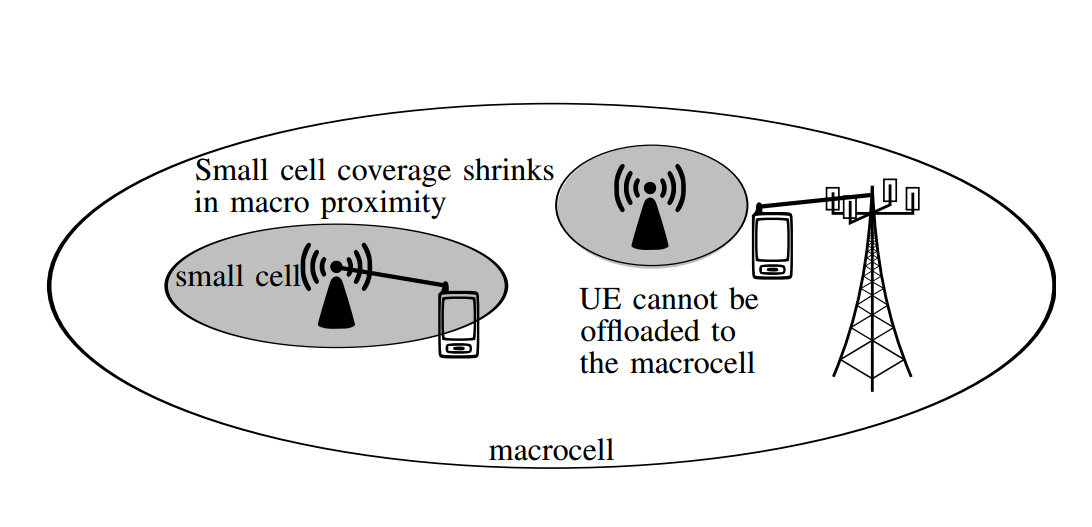
\includegraphics[scale=0.4]{sm_inter}
\centering
\caption{Coverage area reduction of small cell which is close to macro cell due to difference in transmission power.~\cite{main_paper}}
\label{fig:SMI}
\end{figure}

\section{The Application}
\label{sec:TA}

In the early days of wireless communication systems, voice service is the most demanding service with requirements of tens of Kbps per user equipment (UE). However, these days video steaming is the service with high demand requiring tens of Mbps per UE ~\cite{stream_vid}. 
In future, with increase internet of things (IOT) applications such as home automation, monitoring, infrastructure management and autonomous cars etc., the number of UE count increase drastically. 
With the rapid growth in virtual reality (VR) and augmented reality (AR) the requirement for low latency data increase in the gaming applications. 
The streming media services are moving towards higher resolution technologies such as 4K and 8K resolutions require very high data rates ~\cite{youtube}.

The above demands can be meet only by increasing network capacity by atleast 100 folds. This can be achieved by applying modern techniques in wireless communications. Some of them are discussed in section - \ref{sec:TC}.

\section{The Categories}  
\label{sec:TC}
In the survey paper~\cite{main_paper}, authors provided improvements over the existing technologies in three categories as shown in figure-~\ref{fig:NWCP}.

\subsection{More Spatial Efficiency - Network Densification}
\label{subsec:MS}
The current small cell technology is categories as a Type-2 cells, which uses co-channel deployment where small cell BS and Macro cell BS share same frequency bands and is conceived as add to Type-1 cells (Macro cells). These type of small cells are deployed in form of femtocell to improve the performance of the network in 4G LTE. Even though this technology has better frequency utilization, there is a effect of inter-tire interference which can lead to coverage and hand over issues. If the small cell is Close Subscriber Group (CSG) deployment, other UE's cannot connect to this BS can causes interference. These issues can be overcome by using Type-3 cells which cover very small area and however unlike type-2 small cells, these use high frequency bands such as $5Ghz$ and $10Ghz$ to proved network connection to the UE's with non-co-channel deployment. Results in no inter-tire interference.

There are lot of advantages with network densification, as the number of smalls increases and Inter Site Distance(ISD) of each BS reduces. Which leased to high number of geographically separated BSs and simultaneously increase re-usability of the available bandwidth. Which leads to linear increase in the spatial capacity and network capacity.
With reduction in cell size there is also reduction in number of UEs connected, which results in increase in signal quality and network capacity.

With the decrease in the ISD of a cell, travel distance of signal between the BS and UE reduces. With the reduction in the travel distance of the signal, line of sight(LOS) of the received signal is more dominant component than the Non-Line of Sight (NLOS) signal. Which in turn increase the SINR of the received signal.

As the ISD of the cell reduces the distance between the UE and BS reduces. Which reduces the transmission power of the signal while maintaining the SINR. With more number of BS, the number of UEs per base station reduces drastically. In some cases the if there is no UE in the cell, the BS can be placed in the idle mode by making the whole network more energy efficient.

In the survey paper~\cite{main_paper}, authors performed an experiment with changing BS Inter Site Distances (ISDs) from $200m$ to $5m$, which results in $29$ to $46189$ increase in number of BS in $500m$ by $500m$ area of coverage. With $2GHz$ as carrier frequency and $5\%$ of the carrier frequency as available bandwidth i.e., 100MHz. For distribution of UEs, two scenarios are considered. First, uniform distribution and second, half of the UEs are uniformly distributed and remaining are concentrated with in the $40m$ radius with 20 UEs each. 600, 300, and 100 UE densities are considered for the above distributions. The transmission power of each BS is maintained such that the SINR is at 12dB with coverage range of $\sqrt{3}/2$ of the ISD.

\begin{figure}[ht]
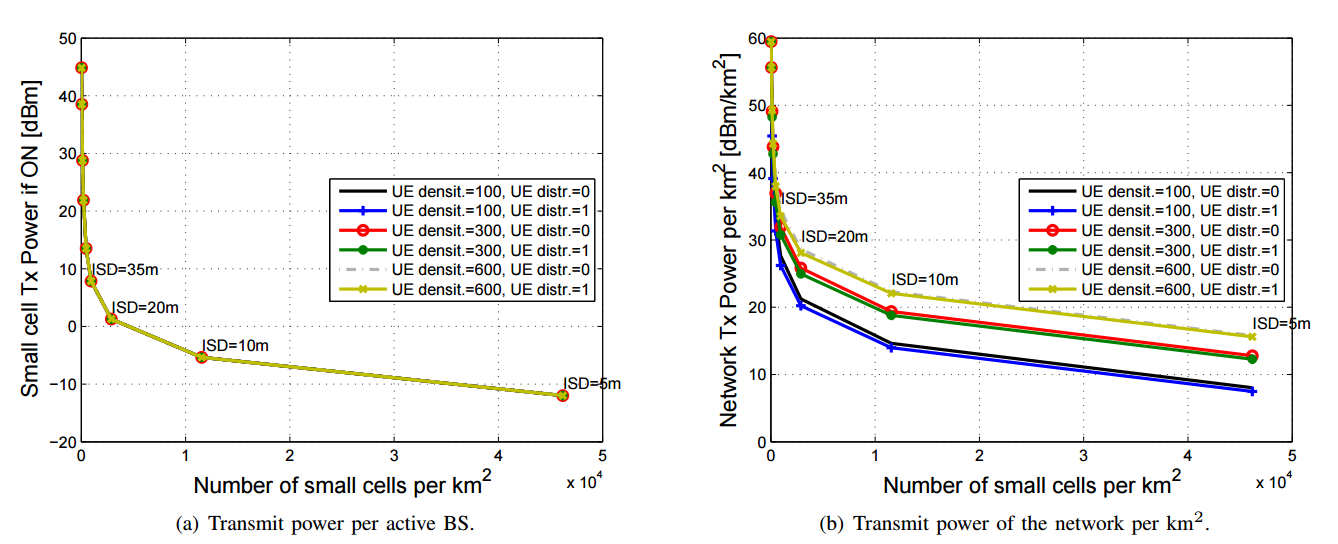
\includegraphics[scale=0.4]{tx_pow}
\centering
\caption{Transmission power of active BS and the total transmission power of the network.~\cite{main_paper}}
\label{fig:TXP}
\end{figure}


From Figure-~\ref{fig:TXP}(a), it can be seen that with the same SINR of 12dB, the transmission power of each BS reduces as the ISD reduces. The reason there is no change in the transmission power with respect to the UE density because power used by the cell is not dependent on the UE density. 0 - indicates uniform UE distribution and 1 - non-uniform UE distribution as discusses above. Figure-~\ref{fig:TXP}(b) shows how the over all network transmission power reduces with reduction in ISD because the reduction in transmission rate per cell outweighs the number of cells active in both uniform and non-uniform UE distribution.

\subsection{More Spectrum - High carrier frequencies}
\label{subsec:MSF}

\begin{figure}[ht]
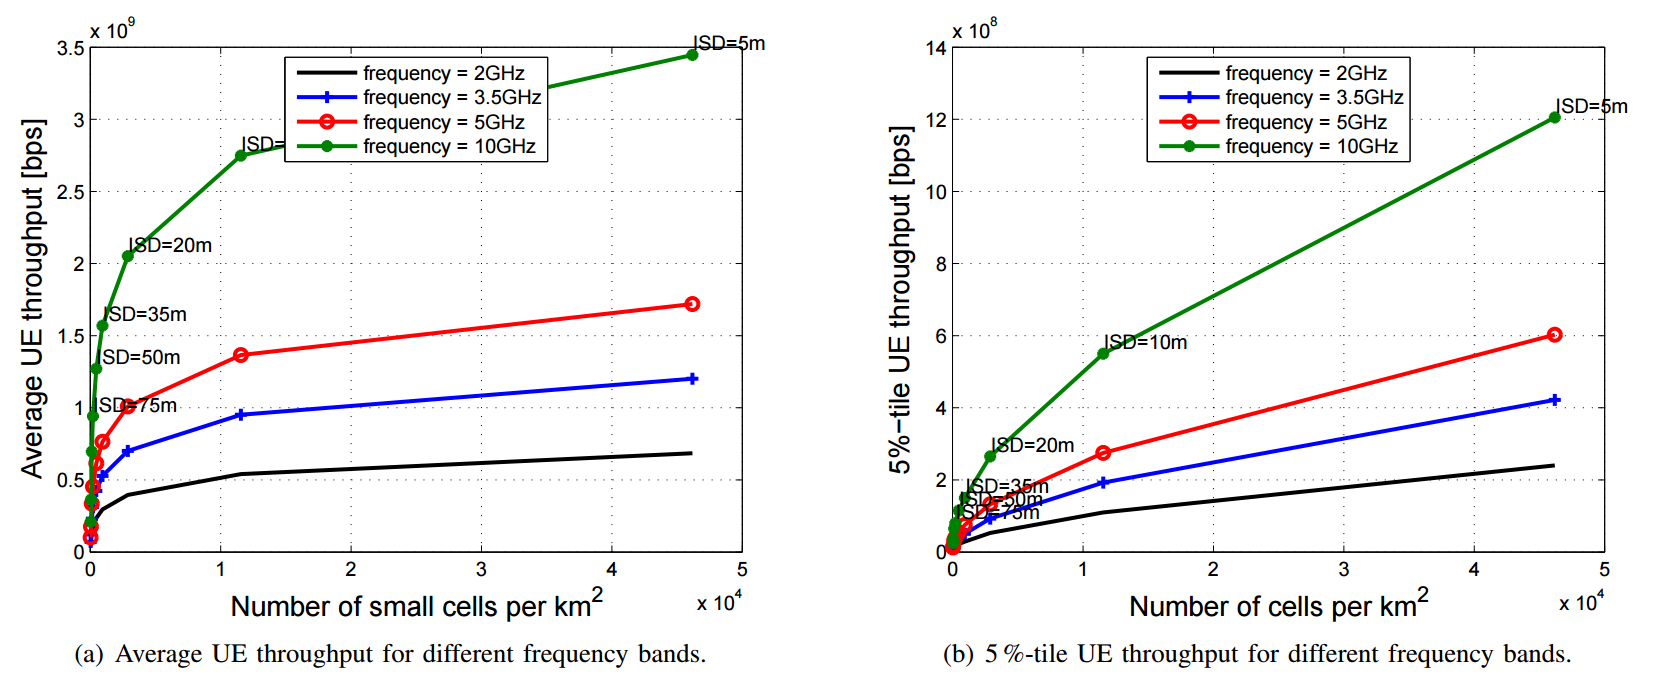
\includegraphics[scale=0.32]{high_freq}
\centering
\caption{Average and $5\%$ UE through for different frequency bands.~\cite{main_paper}}
\label{fig:HF}
\end{figure}

The current generation frequency bands $500MHz$ to $2600MHz$ which are used in wide range of wireless applications such as radio, TV and mobile communications have better long distance propagation properties. Unlike these lower frequency bands due to large propagation loss, higher frequency bands are not been used in macro cell deployments.

With network desification, as the cell size reduses the propagation distance reduces and higher frequency bands can be used as carrier frequencies. Authours in the paper~\cite{main_paper} tested $2Ghz$, $3.5Ghz$, $5Ghz$ and $10Ghz$ with UE density of 300 at different ISDs. From figure-~\ref{fig:HF} it can be seen that the throughput of the UE increases drastically as the carrier frequency band increase from $2Ghz$ to $10Ghz$ with increase in bandwidth from $100MHz$ to $500Mhz$ considering $5\%$ of the carrier frequency as bandwidth. 

\subsection{More Spectral Efficiency - Multi-antenna and Schedulings}
\label{subsec:MSE}

To achieve better spectral efficiency, the authors in the survey paper ~\cite{main_paper} tested beamforming technology with multi-antenna system and different scheduling techniques.

\begin{figure}[ht]
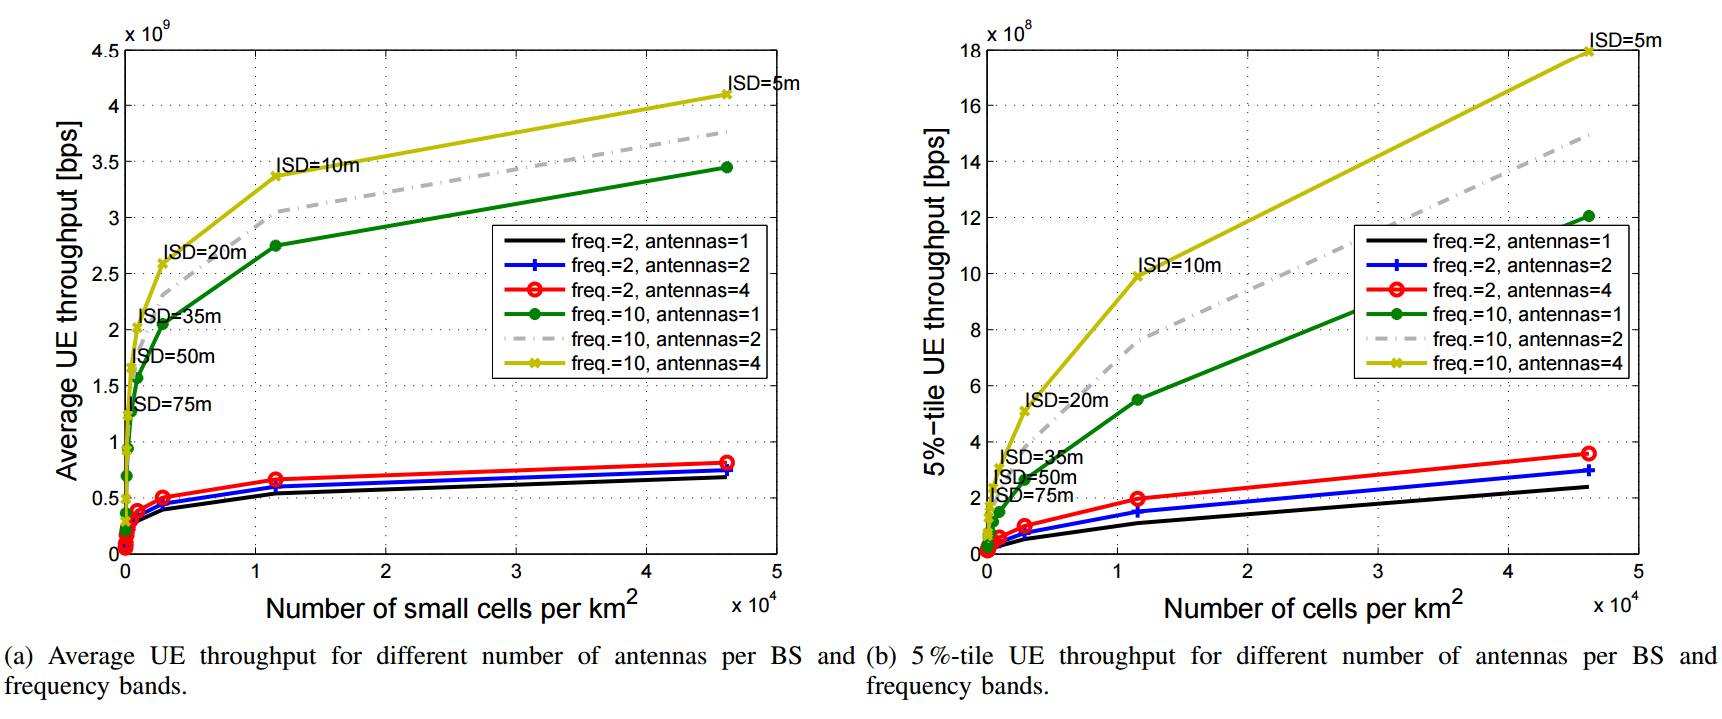
\includegraphics[scale=0.32]{beam_form}
\centering
\caption{Average and $5\%$ UE through for $2Ghz$ and $10Ghz$ with beam forming using 1,2 and 4 antenna at BS.~\cite{main_paper}}
\label{fig:BF}
\end{figure}

The propagation loss increases as the size of ISD increase. It can be over come by using beam forming technology. From figure-~\ref{fig:BF}, it can be seen that at $35m$ ISD the average increase in throughput from $1$ antenna system to $4$ antenna system is $28.11\%$. Where as the edge of the cell, $5\%$-tile, throughput increases by $103\%$ from 1 antenna system to 4 antenna system. It can also be inferred that as the size of the ISD reduces the through put increase, this is because as the size of the ISD reduces the propagation distance reduces and in turn there will be a reduction in propagation loss even in the high frequency bands.

Regrading the schedulling, as the cell size reduces the number of UEs in a cell reduces drastically and there will be less need for complex scheduling techniques used in current generation techniques such as Proportional Fair scheduler (PR). Where the frequency channel is alocated dynamically by measuing the quality of UE. Id the cell size reduces, simple techniques such as Round Robin(RR) scheduler can be used to replace complex schedulers like Proportional Schedulers. It is shown~\cite{main_paper} that as the size of the cell reduces from $200m$ to $20m$, the cell through difference between RR and PR schedulers goes down from $33.33\%$ to $10.5\%$.

From the above simulation results, considering $200m$ ISD and $100MHz$ as the bandwidth. By reducing the ISD to $35m$, we can see UE throughput increase by $7.65Folds$ and by increasing the frequency bands from $2GHz$ to $10GHz$, there is another increase of $5Folds$. This increase already results in reaching $1.27Gbps$ per UE and by using beamforming technology and schedulers, we can see another $2Folds$ increase in average throughput.

\section{The Future}
\label{sec:TF}

It is estimated that by 2020, the number of connected devices per person like to be an average of 5.1 ~\cite{main_paper}. Which in turn increases number of devices in a cell and reduces the average UE throughput. To overcome these short comings, in-future the size of the cell must be reduces more and increase number of BS in the network making it more denser.

The network capacity can be further increased by using higher frequency bands greater than $20GHz$ called mmWaves. Recently ATT published an article ~\cite{att} regarding their ongoing research and developments of using mmWaves for proving high bandwidth data to their customers.

Using multi-antenna technologies such as spatial multiplexing increase the throughput of the cell compare to beamforming, which increases the netowrk capaity lineraly~\cite{satial_mul}.

\section{What We Learn?}
\label{sec:WWL}

Firstly, I learned how important it is to increase the network capacity to meet the feature demands. It is estimated that by 2020, more than $25$ Billion connected devices will in use ~\cite{Gartner} and at an average of 5.1 devices per user ~\cite{frost_sullivan}. To meet these demands the current generation technology are not even close to serve the coming network usage and it need to be improved.

Secondly, I got to learn how the technologies I use in my day to day life work. Especially technologies like spatial multiplexing (MIMO) and network design with different cell types. I also got to learn that as the size of the cell reduces and frequency band increase, there an improvements in throughput, transmission power efficiency and SINR.

Lastly, during the research stage on the survey paper, I came across the recent development in wireless industry and what vendor and network providers are doing to increse the network capacity. Recently major wireless network providers such as Verizon~\cite{verizon5g}, ATT~\cite{att5g} and T-Mobile~\cite{tmobile5g} relese their initiatives regarding their technology and milestones they met moving towards 5G wireless technology. Startups like starry working on providing $1Gbps$ internet for the cities like boston using mmWaves~\cite{techinsider} and recently ATT provided they work on mmWaves with they new service call Airgig~\cite{att}.
\section{Five Most Important Points}
\label{sec:FMIP}

The five important things one need to know from the survey paper are:
\renewcommand{\labelenumi}{\arabic{enumi}}
\begin{enumerate}
   \item Importance of increasing the network capacity for the future demand.
   \item Network Densification is the major paradigm for increasing the network capacity in large increments.
   \item How higher frequencies and smaller cell sizes are more beneficial and have different propagation effects than lower frequencies and macro cells.
   \item In small cells LOS signal dominates compare to NLOS signal.
   \item Inefficiencies of today's small cell network for providing higher throughput.
\end{enumerate}

% Can use something like this to put references on a page
% by themselves when using endfloat and the captionsoff option.
\ifCLASSOPTIONcaptionsoff
  \newpage
\fi

\bibliographystyle{IEEEtran}
\bibliography{biblio}

\end{document}


